\chapter{Structured Learning in Reduced-Operator Model Classes}
\label{ch:structured-learning}

\textbf{Status: proposed learning framework. No trained model, learned impurity
operator, model-class error sequence, or atomistic-to-continuum crossover is
claimed.}

Machine learning enters this program only after the first-principles and
representation problems have been separated. Kohn--Sham DFT supplies a parent
one-particle operator. Projection, retention, energy alignment, and an
admissible identification map then place the pristine and doped operators in a
common represented space. Learning does not replace any of these steps. Its
proposed role is to test how much structure a reduced impurity model requires
in order to approximate the aligned parent operator.

This viewpoint makes the machine-learning question subordinate to a physical
model-selection question. The objective is not simply to fit Kohn--Sham bands
or to emit an unconstrained matrix. It is to compare physically defined
operator classes and determine which additional degrees of freedom materially
reduce a declared discrepancy.

\section{The aligned target precedes learning}

At wavevector $\mathbf k$, let $P$ denote the declared retained-space
projector, and let $H_b^{(P)}(\mathbf k)$ and $H_d^{(P)}(\mathbf k)$ be finite
representations of the pristine and doped Kohn--Sham operators in their retained
spaces. The superscript $(P)$ denotes retention by this projector; the dopant
phosphorus is written $\mathrm P$ when it appears as a species label. Suppose that all prerequisite
geometry, spin, unit, and scalar-energy conventions have been made compatible,
and let
\begin{equation}
  U_d(\mathbf k):
  \mathcal H_b^{(P)}(\mathbf k)
  \longrightarrow
  \mathcal H_d^{(P)}(\mathbf k)
\end{equation}
be an accepted unitary identification. In pristine coordinates, the signed
aligned impurity target is
\begin{equation}
  \Delta H_{d\to b}^{(P)}(\mathbf k)
  =
  U_d^{\dagger}(\mathbf k)\,
  \overline H_d^{(P)}(\mathbf k)\,
  U_d(\mathbf k)
  -
  \overline H_b^{(P)}(\mathbf k),
  \label{eq:learning-aligned-target}
\end{equation}
where the overbar denotes the recorded common scalar-energy convention. This
is one represented target that a reduced model may be asked to reproduce. Its
meaning remains conditional on the retained subspaces and identification
validated in Chapter~\ref{ch:representations-and-alignment}.

A direct supervised objective for a parameterized candidate
$\Delta H_{\theta}(\mathbf k)$ is
\begin{equation}
  \mathcal L_H(\theta)
  =
  \sum_{\mathbf k\in\mathcal K_{\mathrm{train}}}
  \omega_{\mathbf k}
  \left\|
    \Delta H_{d\to b}^{(P)}(\mathbf k)
    -\Delta H_{\theta}(\mathbf k)
  \right\|_{\mathrm F}^{2}.
  \label{eq:learning-operator-loss}
\end{equation}
The sampled set, weights, normalization, units, Fourier convention, and
withheld domain must all be declared. Equation~\eqref{eq:learning-operator-loss}
is a legitimate regression objective, but an unrestricted network that emits
an arbitrary $M\times M$ array would abandon most of the structure established
by the reduction framework.

\section{Structured parameter prediction}

The preferred architecture separates learned parameter prediction from a
deterministic Hamiltonian constructor:
\begin{equation}
  x
  \xrightarrow{\;f_{\phi}\;}
  \boldsymbol\theta(x)
  =\{t_i,\epsilon_i,V_i,\ldots\}
  \xrightarrow{\;\mathcal C\;}
  H_{\phi}(x).
  \label{eq:structured-learning-map}
\end{equation}
Here $x$ denotes declared physical descriptors, $f_{\phi}$ is the learned map,
and $\mathcal C$ constructs an operator in a prescribed model class. Depending
on the class, the constructor can enforce by construction

\begin{itemize}
  \item Hermiticity and the declared spin structure;
  \item lattice, site, and orbital ordering;
  \item crystal or defect symmetries;
  \item prescribed hopping topology and finite interaction range;
  \item locality or a specified form of nonlocality; and
  \item scalar, orbital-dependent, or central-cell potential structure.
\end{itemize}

The descriptors and constructor are part of the scientific model, not neutral
software details. Their invariance, equivariance, boundary, and completeness
properties must therefore be stated. A network cannot repair a descriptor map
that identifies physically distinct environments or a constructor that omits
an essential operator component.

Abstractly, the reduction problem is
\begin{equation}
  \inf_{H\in\mathfrak M}
  d\!\left(\Delta H_{d\to b}^{(P)},H\right),
  \label{eq:model-class-infimum}
\end{equation}
where $\mathfrak M$ is a physically defined reduced-operator class and $d$ is a
discrepancy on compatible representations. Neural optimization is one possible
way to search a class; it does not define the class by itself and does not prove
that the infimum has been found.

\section{Expressiveness through nested model classes}

After embedding all candidates in one comparison space, one may prescribe a
nested hierarchy such as
\begin{equation}
  \mathfrak M_{\rm EMT}
  \subseteq
  \mathfrak M_{\rm scalar}
  \subseteq
  \mathfrak M_{\rm orbital}
  \subseteq
  \mathfrak M_{\rm finite\mbox{-}range}
  \subseteq
  \mathfrak M_{\rm NN}.
  \label{eq:learning-model-hierarchy}
\end{equation}
This nesting is a contract to be demonstrated, not inferred from the class
names. For example, the EMT operator requires an explicit continuum-to-atomistic
embedding before it can be a member of a lattice comparison class, and a
structured neural constructor contains the earlier classes only if its
parameterization can reproduce them exactly.

For a nonzero target, define the best normalized represented-operator error
\begin{equation}
  \epsilon(\mathfrak M)
  =
  \inf_{H\in\mathfrak M}
  \left(
  \frac{
    \sum_{\mathbf k\in\mathcal K}
    \omega_{\mathbf k}
    \left\|\Delta H_{d\to b}^{(P)}(\mathbf k)-H(\mathbf k)\right\|_{\mathrm F}^{2}
  }{
    \sum_{\mathbf k\in\mathcal K}
    \omega_{\mathbf k}
    \left\|\Delta H_{d\to b}^{(P)}(\mathbf k)\right\|_{\mathrm F}^{2}
  }
  \right)^{1/2}.
  \label{eq:model-class-error}
\end{equation}
A zero-target case requires an absolute scale rather than this normalization.
For genuinely nested classes, the exact infima obey
\begin{equation}
  \epsilon_1\geq\epsilon_2\geq\cdots\geq\epsilon_J.
\end{equation}
Numerically obtained training errors need not obey or attain this sequence
because optimization, sampling, regularization, and finite precision introduce
additional error. Approximation error, estimation or generalization error, and
optimization error must therefore be reported separately whenever the evidence
supports that decomposition.

The useful scientific information lies in the changes between adjacent
classes. Consider, for example, the scalar onsite hypothesis
\begin{equation}
  [\Delta H]_{i\alpha,j\beta}
  \approx
  V_i\,\delta_{ij}\delta_{\alpha\beta}.
  \label{eq:scalar-onsite-hypothesis}
\end{equation}
If allowing orbital dependence yields no material improvement under controlled
optimization and withheld evaluation, then the tested evidence does not require
orbital dependence at that scale. If allowing off-site blocks yields a large,
reproducible reduction, nonlocality is implicated as an important correction
within the tested representation. Neither observation is automatically a
universal physical conclusion: both remain conditional on the target,
embedding, metric, domain, and tolerances.

A range hierarchy may impose
\begin{equation}
  [\Delta H]_{i\alpha,j\beta}=0
  \quad\text{when}\quad
  \lvert\mathbf R_i-\mathbf R_j\rvert>R
\end{equation}
and evaluate $\epsilon(R)$. This tests the represented spatial range of the
impurity operator. The attribution of a nonlocal matrix element to a radius,
its periodic-image treatment, and the tested supercell sequence must be fixed
before $\epsilon(R)$ is interpreted physically.

\section{A learned reference for the continuum crossover}

The continuum question can be phrased as the emergence, over a declared
exterior domain, of a smaller effective-mass operator class. A screened
Coulomb donor term has the asymptotic form
\begin{equation}
  V_{\rm EMT}(r)
  \sim
  -\frac{e^2}{4\pi\epsilon_0\epsilon_r r},
\end{equation}
but the physical specification cautions that the primary neutral P:Si
supercell perturbation must not be silently relabelled as an ionized donor-core
potential. The charge-state interpretation and screening content must be
established before this form is used as a target.

Let $P_{>R}$ denote the declared projector onto an exterior atomistic region,
and let $H_{\mathfrak M}^{\ast}$ be a best or controlled approximate fit in
class $\mathfrak M$. One class-relative exterior discrepancy is
\begin{equation}
  \eta_{\mathfrak M}(R)
  =
  \left\|
    P_{>R}
    \left(\Delta H_{d\to b}^{(P)}-H_{\mathfrak M}^{\ast}\right)
    P_{>R}
  \right\|,
  \label{eq:class-exterior-error}
\end{equation}
with cross-boundary blocks assessed separately as required by the crossover
contract in Chapter~\ref{ch:model-reduction}. A highly expressive structured
model can serve as a reference class. If its validated exterior error is much
smaller than that of EMT near the impurity but offers no material advantage
beyond a radius, that pattern can contribute to an operational crossover
assessment.

Agreement between two fitted errors is not sufficient by itself. Both models
must satisfy the prespecified absolute tolerances; optimization and
sampling errors must be controlled; and the exterior and cross-coupling
criteria must hold for every tested larger radius. A learned reference therefore
does not establish EMT by assumption. It provides a more expressive comparator
within a larger body of crossover evidence.

\section{Learning the residual beyond a continuum model}

A particularly interpretable construction assigns the known continuum model as
a baseline and learns only a correction:
\begin{equation}
  \Delta H_{d\to b}^{(P)}
  =
  \Delta H_{\mathrm{EMT}\to\mathrm{ret}}
  +\delta H_{\phi}
  +E_{\phi},
  \label{eq:emt-residual-decomposition}
\end{equation}
where $\Delta H_{\mathrm{EMT}\to\mathrm{ret}}$ denotes the continuum operator
after a validated embedding into the retained atomistic space, $\delta H_{\phi}$ is a constrained
atomistic correction, and $E_{\phi}$ is the remaining represented residual.
One proposed objective is
\begin{equation}
  \mathcal L_{\rm residual}(\phi)
  =
  \left\|
    \Delta H_{d\to b}^{(P)}
    -\Delta H_{\mathrm{EMT}\to\mathrm{ret}}
    -\delta H_{\phi}
  \right\|_{\mathrm F}^{2}
  +\lambda\,\mathcal R(\delta H_{\phi}),
  \label{eq:residual-learning-loss}
\end{equation}
where $\mathcal R$ is a declared complexity or locality penalty. The value of
$\lambda$ changes the fitted model and must be selected without using withheld
acceptance data.

This formulation asks which smallest admissible correction to effective-mass
theory is required relative to the aligned Kohn--Sham target. The correction can
be decomposed by onsite contribution, orbital dependence, off-diagonal orbital
mixing, hopping range, symmetry channel, and radial decay. Such decompositions
are more interpretable than a validation score alone, provided that their gauge
and localization dependence is also reported.

\section{Composite objectives and acceptance}

Operator fidelity can be combined with other declared reduction quantities:
\begin{equation}
  \mathcal L
  =
  \lambda_H\mathcal L_H
  +\lambda_{\rm spec}\mathcal L_{\rm spec}
  +\lambda_{\Pi}\mathcal L_{\Pi}
  +\lambda_{\rm loc}\mathcal L_{\rm loc}
  +\lambda_{\rm EMT}\mathcal L_{\rm EMT}.
  \label{eq:composite-learning-loss}
\end{equation}
For example, a normalized operator term may be
\begin{equation}
  \mathcal L_H
  =
  \frac{
    \sum_{\mathbf k}\omega_{\mathbf k}
    \left\|H_{\rm target}(\mathbf k)-H_{\phi}(\mathbf k)\right\|_{\mathrm F}^{2}
  }{
    \sum_{\mathbf k}\omega_{\mathbf k}
    \left\|H_{\rm target}(\mathbf k)\right\|_{\mathrm F}^{2}
  },
\end{equation}
a spectral term may be
\begin{equation}
  \mathcal L_{\rm spec}
  =
  \sum_{n,\mathbf k}w_{n\mathbf k}
  \left(E_{n\mathbf k}^{\rm target}-E_{n\mathbf k}^{\phi}\right)^2,
\end{equation}
and a locality penalty in real space may be
\begin{equation}
  \mathcal L_{\rm loc}
  =
  \sum_{\mathbf R}w(\mathbf R)
  \left\|H_{\phi}(\mathbf R)\right\|_{\mathrm F}^{2},
\end{equation}
where $w(\mathbf R)$ increases with separation.

A weighted sum is an optimization device, not automatically an acceptance
rule. Its weights can hide a failed criterion behind success on another.
Final model selection should therefore retain the separate metrics and apply
the prespecified admissible-set criteria developed in
Chapter~\ref{ch:model-reduction}. Symmetry, Hermiticity, and other exact
requirements should be enforced by the constructor where possible rather than
encouraged only by soft penalties.

\section{Joint learning of identification and reduction}

A more ambitious problem optimizes both the coordinate identification and the
reduced operator:
\begin{equation}
  \inf_{\substack{U\in\mathcal G\\H\in\mathfrak M}}
  d\!\left(
    U^{\dagger}\overline H_d^{(P)}U-
    \overline H_b^{(P)},
    H
  \right),
  \label{eq:joint-gauge-model-problem}
\end{equation}
where $\mathcal G$ is an admissible identification class. A learned unitary may
be parameterized through an anti-Hermitian generator,
\begin{align}
  A_{\psi}^{\dagger}(\mathbf k)&=-A_{\psi}(\mathbf k),\\
  U_{\psi}(\mathbf k)&=\exp A_{\psi}(\mathbf k),
\end{align}
so that unitarity holds by construction. The joint sampled objective would then
compare
\begin{equation}
  U_{\psi}^{\dagger}(\mathbf k)
  \overline H_d^{(P)}(\mathbf k)
  U_{\psi}(\mathbf k)
  -\overline H_b^{(P)}(\mathbf k)
\end{equation}
with $\Delta H_{\phi}(\mathbf k)$.

This problem exposes the search for both coordinates and a simple operator in
those coordinates, but it is generally less identifiable than either problem
alone. A sufficiently expressive reduced model can absorb an incorrect
identification, while a flexible identification can make an operator appear
artificially simple. Low training loss would not establish physical
correspondence. Any future joint method therefore requires independent overlap,
locality, symmetry, smoothness, and gauge-equivariance constraints together
with controlled synthetic recovery tests.

The safer progression and the staged escalation of model expressiveness are
summarized in Figure~\ref{fig:structured-learning-process}. Joint optimization
over $U$ and $H$ remains a later proposed investigation, not the first learning
experiment.

\begin{figure}[p]
  \centering
  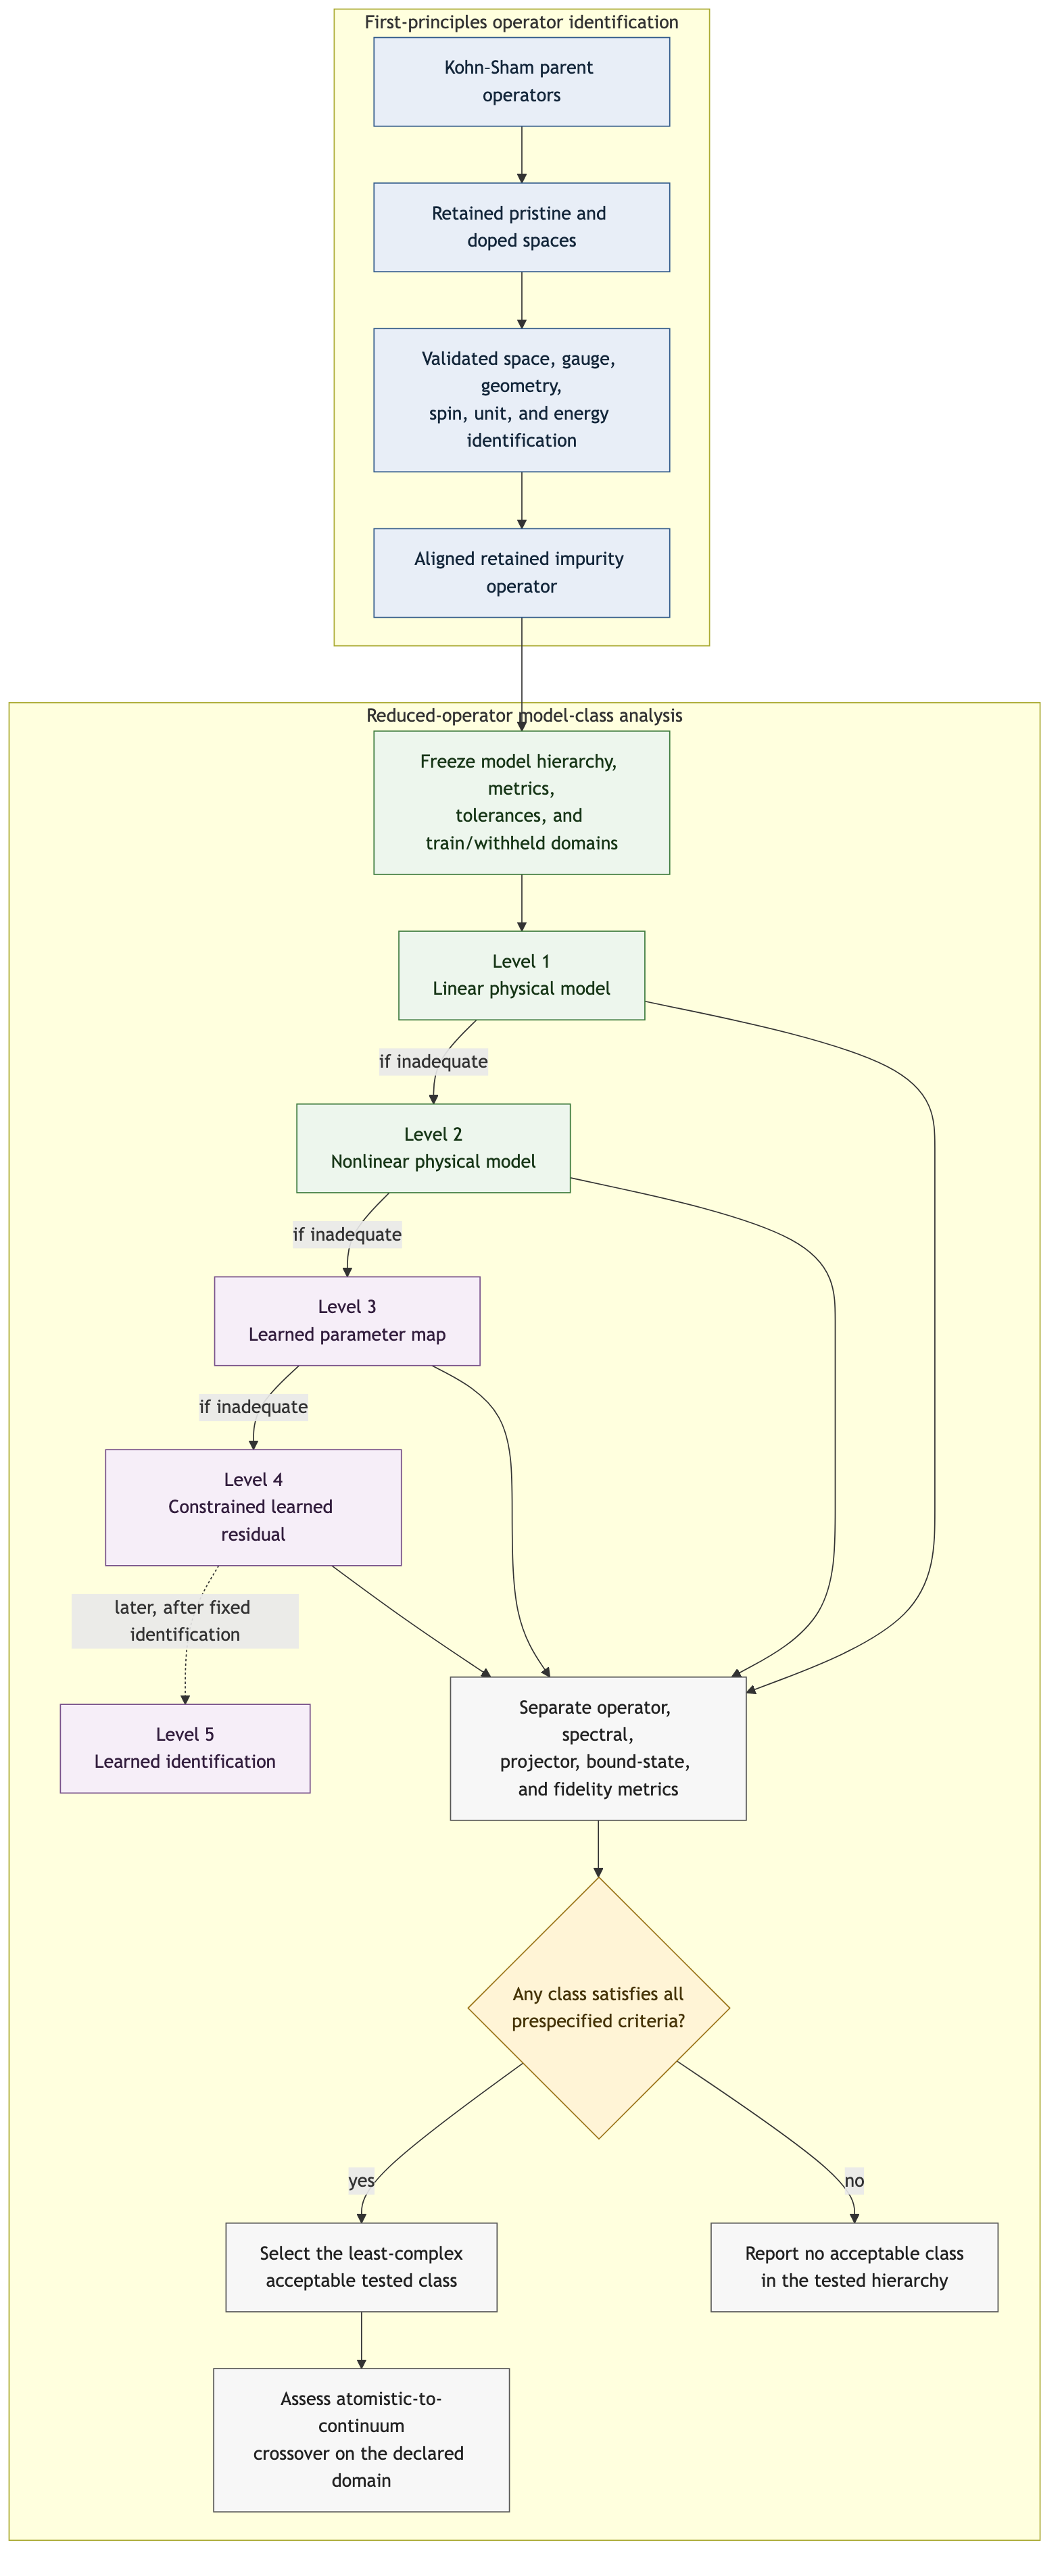
\includegraphics[
    width=\textwidth,
    height=0.80\textheight,
    keepaspectratio
  ]{figures/structured-learning-process.png}
  \caption{Proposed operator-identification and structured-learning process.
  Solid arrows show the fixed-identification progression and escalation through
  increasingly expressive model classes when a simpler tested class is
  inadequate. The dotted arrow marks learned identification as deferred work.
  The editable Mermaid source is retained in
  \texttt{figures/structured-learning-process.mmd}.}
  \label{fig:structured-learning-process}
\end{figure}

\section{A staged computational progression}

The proposed progression introduces flexibility only when a simpler level is
shown to be inadequate under its declared tests.

\begin{description}
  \item[Level 1: linear physical model.] Use fixed stencils or a linear
    Slater--Koster or tight-binding parameterization and solve by linear least
    squares when the model permits it.
  \item[Level 2: nonlinear differentiable physical model.] Retain a
    deterministic Hamiltonian constructor while optimizing nonlinear physical
    parameters.
  \item[Level 3: learned parameter map.] Introduce a neural map only when
    admissible parameters must depend nonlinearly on a declared local
    environment.
  \item[Level 4: learned residual operator.] Fit the constrained correction
    beyond simpler accepted physical classes and decompose the residual by
    physical operator content.
  \item[Level 5: learned identification.] Only after fixed-identification
    behavior is understood, investigate optimization over an admissible gauge
    or identification manifold.
\end{description}

Failure can be informative. Success at Level~1 would show that the tested target
requires no learned parameter map for the declared use. A gain at Level~2 would
show the value of nonlinear parameter dependence within the same constructor.
A reproducible gain from a structured learned model would identify missing
expressiveness in the simpler tested classes. Failure of an expressive model
under fixed constraints may indicate incompatible constraints, inadequate
descriptors, insufficient data, or optimization failure; these alternatives
must be distinguished before a scientific interpretation is assigned.

\section{Scientific question and evidence boundary}

The proposed central question is
\begin{quote}
What is the lowest-complexity operator class in which the aligned retained
Kohn--Sham impurity problem is representable within prespecified tolerances for
a declared use?
\end{quote}
For each candidate class $\mathfrak M$, let $\mathfrak A_{\mathfrak M}$ be the
subset satisfying every prespecified operator, spectral, projector, bound-state,
fidelity, and exact structural criterion applicable to the declared use. One
formal expression is
\begin{equation}
  \mathfrak M^{\ast}
  \in
  \arg\min_{\substack{\mathfrak M\in\mathfrak H\\
                      \mathfrak A_{\mathfrak M}\ne\varnothing}}
  \operatorname{complexity}(\mathfrak M).
  \label{eq:minimal-operator-class}
\end{equation}
The condition $\epsilon(\mathfrak M)\leq\epsilon_{\rm target}$ may define the
operator-error component of $\mathfrak A_{\mathfrak M}$, but it cannot replace
the other required criteria. The candidate hierarchy $\mathfrak H$, complexity
ordering, metrics, tolerances, training protocol, and withheld validation domain
are frozen before selection. If no tested class passes, no acceptable class has
been identified within the tested hierarchy.

A constrained neural model is thus an expressive comparator, not the central
physical model and not an infallible oracle. It can help test whether a simpler
physical class has exhausted its representational capacity only when
optimization adequacy and generalization have independent evidence. The
complete proposed pipeline is the process shown in
Figure~\ref{fig:structured-learning-process}.

This framing makes the learning component useful because it is accountable to
the operator-identification framework. It asks not whether a flexible model can
fit a matrix, but which physically interpretable restrictions can be retained
without losing the parent information required for the intended reduction.
